\documentclass[10pt,twocolumn]{article}
\usepackage{multicol}
\usepackage{graphicx}

% definitions
\def \tool {InputFinder}  

\begin{document}

\twocolumn[{%
  \centering
  \large \textbf{InputFinder: Reverse Engineering Closed Binaries via Side Channels} \\[2em]
  Bogdan Copos, University of California, Davis\\
  Praveen Murthy, Fujitsu Laboratories of America \\[4em]
}]


\begin{abstract}
Valid input and test suites are crucial to dynamic program analysis techniques.
Without extensive testing of the program, bugs may be omitted.
While fuzzing and symbolic execution can be successful in finding input, both approaches have limitations.
To date, there is no alternative method for generating input for closed (source) binaries.
In this paper we present an architecture and source code independent, instrumentation-free technique and its implementation, \tool{}, for generating valid input for closed stripped binaries.
\tool{} exploits side channels to automatically build valid user-input allowing for more extensive testing.
Additionally, \tool{} can determine expected input size and make inferences about input types (e.g. alphabetic, numeric, alphanumeric, etc.).
\end{abstract}

\section{Introduction}

Software testing is an expensive and labor intensive process.
For many years, researchers have explored both static and dynamic methods for analyzing programs.
While static analysis is the more thorough approach, dynamic testing is often preferred due to its time efficiency.
Dynamic testing heavily depends on availability of input or test suites.
Without input, the program cannot be properly tested and bugs may be omitted.
While valid input can be learned from software documentation or source code, when such information is not available, other methods must be used.
Automated dynamic analysis techniques such as fuzzing and symbolic execution attempt to generate input for a given program.
Currently these are the only two options available and both approaches present discouraging limitations.

In this paper, we introduce a third method for generating valid user-input for closed stripped binaries. 
Our method exploits side channels to build valid input for closed binaries.
Specifically, our method relies on hardware instruction counter registers.
We show that by measuring the number of user-land instructions retired and comparing them between different executions of the program with various input, it is possible to learn the program's expected input.
We also present an implementation of our method, \tool{}.

The contributions of this paper are as follows:
\begin{itemize}
	\item We introduce a new approach to automatically generate input valid strings for unknown, closed-source binaries by leveraging hardware instruction counters. Our method relies on observing additional instructions executed by programs during their input validation process to learn valid input strings.
	\item We implement the method presented and evaluate it using example binaries published by DARPA as part of the 2014 Cyber Grand Challenge competition. Additionally, we compare our approach to the manual process used by a security specialist to crack a binary as part of a job interview.
\end{itemize}

The paper is organized as follows.
Section 2 covers background information.
Section 3 discusses related works and differences with respect to the presented method.
In Section 4 our method is explained.
Section 5 describes evaluation of the method presented and the results.
In Section 6 we discuss future work and limitations of the presented work.

\section{Background}
 
\subsection{Side Channels}

Side channels are streams of information that can be retrieved from the hardware of a device running a given program.
This information can be used to learn more about the program's internals.
Side channels have been widely explored by security researchers in order to exploit weaknesses in programs.
In cryptography, side channel attacks exploit such information channels to break crypto systems rather than applying traditional brute force or reverse engineering techniques.
Recently, side channel attacks, such as OpenSSL's CREAM cache timing attack have made headlines. [CITE]
Similar to CREAM and other side channel attacks, the technique discussed in this paper exploits such information channels to generate valid input for binaries.

\subsection{Hardware counter registers}

Most modern microprocessors have a set of special-purpose registers built to store the counts of hardware events.
Each counter can be programmed to measure specific events such as cache misses, floating point operations, and even instructions executed.
Utilities, such as Linux/Unix `perf', take advantage of such hardware counters in order to provide developers with useful information about a program's performance.
`perf' is a tool which allows developers to specify the desired hardware event they wish to measure.
Once events have been s�elected, `perf' interacts with kernel modules to program the hardware counters accordingly.
In this work, we use `perf' to count the number of \textbf{user-land} instructions executed as a program is tested with various input.
The number of total instructions retired oscillates significantly for a binary from execution to execution.
This phenomena reflects fluctuations in instructions executed by the kernel depending on the state of the machine due to cache-misses and other events.
Since we rely on this count, such variations are problematic.
However, the number of user-land instructions only varies by one instruction on average, giving us a reliable counter.

\section{Previous Work}

Fuzzers are a popular choice amongst software testers.
They are easy to use and have produced good results in the past.
There are two classes of fuzzers: black box fuzzers and white box fuzzers.
In black box fuzzing, testing is based on randomly generating input and observing output to identify problems.
No program specifications or knowledge of the input format is available in such cases.
On the other hand, in white box fuzzing, inputs are used to gather symbolic constraints which are in turn systematically negated and solved to produce more inputs.
White box fuzzing differs from black box fuzzing in that it uses the program's feedback to make inferences about valid input and use constraint solvers to generate more input.
Both fuzzing approach have limitations.
Since black box fuzzing is completely random, its effectiveness is limited, especially with respect to exercising programs.
White box fuzzing can attain better code coverage but can be slow.
[MAYBE TALK ABOUT FUZZING RESULTS, CITATIONS]

Symbolic execution is another method used for generating valid input.
In symbolic execution, an interpreter gathers constraints related to input throughout the program's execution, rather than using the provided input.
At the end of the execution, a constraint solver takes the constraints gathered and outputs valid program input.
Symbolic execution has been studied extensively and has been proved effective [CITE].
[TALK ABOUT ONE OF THE CITATIONS]
Despite positive results, symbolic execution has a fundamental limitation with respect to constraint solving.
While symbolic execution engines perform well when constraints are linear, non-linear constraints greatly impact efficiency.
Furthermore, there is no autonomous symbolic execution engine.
All symbolic executioners today require some instrumentation of the program to determine the program's input buffer.
Some symbolic execution engines even require source code, which is not always available to the tester.

Side channel attacks and citations\ldots

The method presented in this paper takes advantage of hardware counters to observe program's behavior and automatically build valid input.
As opposed to fuzzers, where input is randomly generated, this approach uses side channels to intelligently compose valid program input.
Also, unlike symbolic execution, this approach is not hindered by constraint solver limitations and does not require any instrumentation or source code.

\section{Methodology}

The majority of software programs accept input, perform transformations on the input and output the result.
However, most programs do not accept completely random input.
Input usually passes through an input validation filter.
Such filters are snippets of code responsible for distinguishing between valid or good input (i.e. input the program was constructed to understand) and bad input (i.e. input which is not useful or does not follow the desired format).
Although validation mechanisms can be very sophisticated, they are often a combination of string comparisons and conditional statements.
Our method exploits the presence (or lack) of these additional instructions during an execution to make inferences about the program's validation mechanism.
Specifically, we test the program with different input and compare the number of retired user-land instructions executed.
Assuming most input is invalid, our method observes differences in the number of instructions executed (from the norm) to detect input which does pass the validation mechanism.

We present \tool{} an implementation of the method described above.
Given a closed binary, \tool{} can build valid input, inform the tester about the type of acceptable input, and determine input buffer size.

\subsection{Finding Valid Input}

\begin{figure*}[t]
\centering
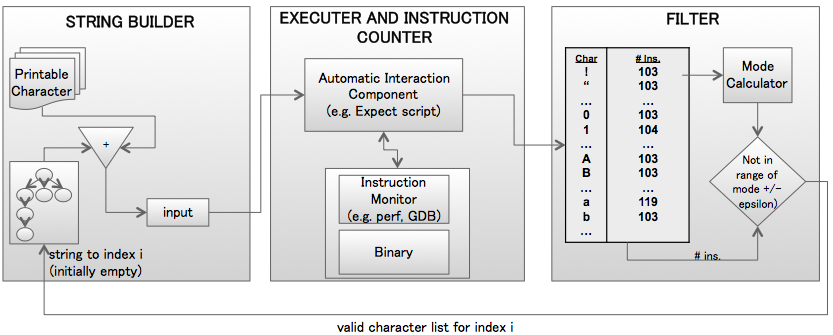
\includegraphics[height=2.5in,width=6.5in]{architecture.png}
\label{fig:architecture}
\caption{}
\end{figure*}

In order to build valid input for a given program, \tool{} measures the number of user-land instructions retired during the program's execution using the `perf' utility.
Specifically, \tool{} observes differences in the number of instructions executed as a result of different input.
Generating valid input strings is a recursive two-step process.
\tool{} works by identifying valid characters for each index \textit{i}, starting with \textit{i}=0 and incrementally building valid input strings using the discovered characters.
Figure~\ref{fig:architecture} shows the overall architecture of \tool{}.

\subsubsection{Finding Valid Characters}

The process of finding valid characters for a given index is composed of two stages: the testing stage and the filtering stage.
During the testing stage, the program is executed with `perf' and being provided as input, all of the printable characters, one at a time.
Once the program has processed the input and is waiting for more input, the program is stopped.
The automatic interaction with the program is performed using `Expect', an extension to the `Tcl' scripting language [CITE]
In our implementation, each printable character results in a different program execution.
At the end of each execution, the number of instructions retired is outputted by `perf'.
This information is saved in a dictionary as a tuple of the format ( <printable character> , <number of instructions> ).
As mentioned earlier, the differences in the number of instructions between various printable characters reflect different execution paths taken during the validation process.

The filtering stage is responsible for identifying characters which are highly likely to be part of a valid input string at a given index.
Using the dictionary data obtained from the testing stage, the number of instructions retired are analyzed.
First, the mode of the number of instructions executed is calculated.
The filtering of possible valid characters for a given index \textit{i}, of an input string \textit{s}, is based on the assumption that the majority of printable characters \textit{c} do not belong at index \textit{i} of string \textit{s} (i.e. \textit{c} $\notin$ \textit{s[i]}).
Therefore, valid characters are defined as any printable character for which the number of instructions retired is outside the mode.

While the initial reaction is to expect a valid character to result in more instructions executed than a non-valid character, this is not always the case.
As discussed earlier, the input validation mechanism can be complex and can vary in behavior.
The validation mechanism may verify input against all accepted input strings before denying the provided input.
Such a scenario results in more instructions executed for invalid input than valid input.

When no valid characters are identified as part of the filtering stage and the current index is greater than 0, the end of a valid input string has been reached. If the index is 0 and no valid characters have been found, the given binary has no predefined input commands.

\subsubsection{Building Input Strings}

\begin{figure*}[t]
\centering
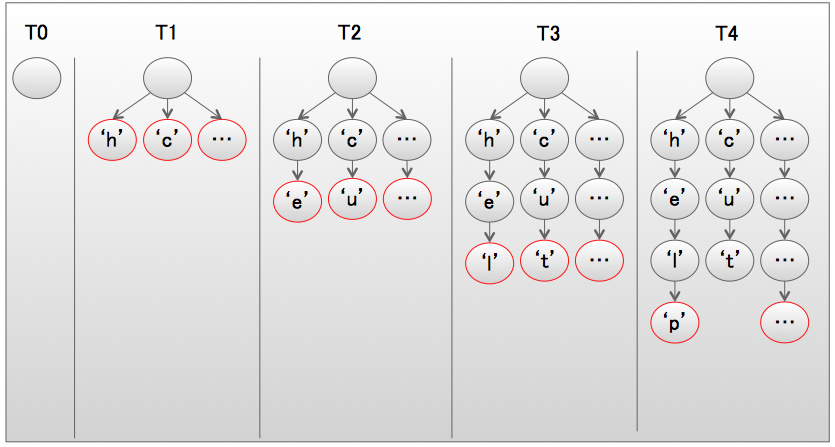
\includegraphics[height=2in,width=6.5in]{string_builder.png}
\label{fig:string_builder}
\caption{}
\end{figure*}


Building valid input strings is a recursive process.
Starting with an empty string and index 0, \tool{} tries to find valid characters at each index and incrementally builds valid input strings.
More specifically, using the character finding technique described previously, relevant characters for index 0 are identified.
The task is forked \textit{n} times, where \textit{n} is the number of characters found at the current index (i.e. index 0).
Each child task is assigned one of the \textit{n} characters and is responsible for finding valid characters at the next index.
These steps are repeated until no valid characters are found, marking the end of the input string.
Figure~\ref{fig:string_builder} depicts the process.

\subsection{Finding Desired Input Size}

The same side channels can be used to detect the expected size of the program's input or even the program's input buffer.
Most programs are designed to read a predefined number of bytes from the source of input and store them in a buffer.
Depending on the implementation, when a program is given more input than the size of the buffer, additional instructions may be executed.
Regardless of the number of instructions executed, the behavior of the program changes.
A program may exit when the number of provided bytes is larger than expected.
Similarly, once the input buffer size limit has been reach, a program may check to see if the next byte is a newline or EOF.
Some methods, such as C's `fgets()' function, read character by character [EXPLAIN]
Our method observes such differences in the number of user-instructions retired as the program is given increasingly larger input.

To start, \tool{} finds the set of all invalid characters for index 0 of all input strings and picks one at random.
The character selected is used to build invalid input strings of various sizes.
It is crucial to use invalid input to avoid noisy fluctuations in the number of instructions executed due to valid input processing.
Initially, the program is executed with short length input strings (i.e. two and three characters).
The number of user-land instructions executed during these two executions are recorded.
These two values may be equal or differ, depending on the program's logic.
If the two values are equal [EQUAL]
The two values can also differ because... [DIFFERENT]



\subsection{Classifying Input}

Our method is also capable of classifying the input discovered.
Generated input strings are classified in three categories: alphabetic, numeric, alphanumeric.
Similarly, the classification algorithm detects special characters.
Once enough input strings have been identified, \tool{} uses the categorization data to generalize about the type of input the program accepts.
Such information is valuable especially in cases where the inputs discovered are all numeric or contain (one or more) special characters.
Having learned such information about the program, the testing platform (e.g. fuzzer) can be adjusted to proceed accordingly.

\section{Evaluation and Results}

\tool{} was tested on [NUMBER] closed-source binaries to measure its effectiveness.
The results are summarized in Figure [FIGURE].
Out of the total [NUMBER] binaries, [NUMBER2] had predefined accepted input strings.
\tool{} found 100\% of the input strings for [NUMBER3]...
[CONTINUE].

Additionally, our method was tested on a binary used for technical interviews.
The binary was designed as a reverse engineering challenge for interviewers.
To pass the challenge, the interviewer has to crack the secret passcode to the program.
A blog post describes the manual process used to crack the password [CITE].
The manual process is tedious.
As described in the blog post, the cracking of the binary can take several hours and requires advanced skills and years of background knowledge.
\tool{} cracked the binary in a matter of minutes automatically, proving itself as a useful tool not only finding valid input but also cracking passwords.

\section{Future Work and Limitations}

The current implementation uses `perf' to count instructions, which outputs only when the program executed exits.
As a result, the tested program must be executed once with every new input string.
This is not only a slow and inefficient process but also hinders the ability to crack programs which randomly generate passwords at execution time.
In the future, we'd like to explore methods which allow sampling of instruction count during runtime.

While the method presented in this paper has many advantages, it also has a few limitations.
For certain programs that allow any input, such as an echo server, our method is not any more efficient than a fuzzer.
Additionally, our method cannot handle cases in which input is composed of multiple inter-dependent fields or when programs validate input fields out of order.

\section{Conclusions}



\end{document}
